\documentclass{article} % For LaTeX2e
\usepackage{nips13submit_e,times}
\usepackage{hyperref}
\usepackage{url}
\usepackage{amsmath}
\usepackage{amssymb}
\usepackage{natbib}
\usepackage{graphicx}
%\documentstyle[nips13submit_09,times,art10]{article} % For LaTeX 2.09

% \DeclareMathOperator{\Sample}{Sample}
\let\vaccent=\v % rename builtin command \v{} to \vaccent{}
\renewcommand{\v}[1]{\ensuremath{\mathbf{#1}}} % for vectors
\newcommand{\gv}[1]{\ensuremath{\mbox{\boldmath$ #1 $}}} 
% for vectors of Greek letters
\newcommand{\uv}[1]{\ensuremath{\mathbf{\hat{#1}}}} % for unit vector

\let\underdot=\d % rename builtin command \d{} to \underdot{}
\renewcommand{\d}[2]{\frac{d #1}{d #2}} % for derivatives
\newcommand{\dd}[2]{\frac{d^2 #1}{d #2^2}} % for double derivatives
\newcommand{\pd}[2]{\frac{\partial #1}{\partial #2}} 
% for partial derivatives
\newcommand{\pdd}[2]{\frac{\partial^2 #1}{\partial #2^2}} 
% for double partial derivatives
\newcommand{\pdc}[3]{\left( \frac{\partial #1}{\partial #2}
 \right)_{#3}} % for thermodynamic partial derivatives
\newcommand{\ket}[1]{\left| #1 \right>} % for Dirac bras
\newcommand{\bra}[1]{\left< #1 \right|} % for Dirac kets
\newcommand{\braket}[2]{\left< #1 \vphantom{#2} \right|
 \left. #2 \vphantom{#1} \right>} % for Dirac brackets
\newcommand{\matrixel}[3]{\left< #1 \vphantom{#2#3} \right|
 #2 \left| #3 \vphantom{#1#2} \right>} % for Dirac matrix elements

\newcommand{\exval}[1]{\left\langle #1 \right\rangle} % for angle-bracket expectation values

\newcommand{\abv}[1]{\lvert #1 \rvert} % for absolute values

\title{Criticality in neural networks paper title}


\author{
Paul Rozdeba%\thanks{ Use footnote for providing further information
%about author (webpage, alternative address)---\emph{not} for acknowledging
%funding agencies.} \\
\\
Department of Physics\\
University of California, San Diego\\
La Jolla, CA 92093 \\
\texttt{prozdeba@physics.ucsd.edu} \\
\And
Forrest Sheldon \\
Department of Physics\\
University of California, San Diego\\
La Jolla, CA 92093 \\
\texttt{forrestemail@physics.ucsd.edu} \\
}

% The \author macro works with any number of authors. There are two commands
% used to separate the names and addresses of multiple authors: \And and \AND.
%
% Using \And between authors leaves it to \LaTeX{} to determine where to break
% the lines. Using \AND forces a linebreak at that point. So, if \LaTeX{}
% puts 3 of 4 authors names on the first line, and the last on the second
% line, try using \AND instead of \And before the third author name.

\newcommand{\fix}{\marginpar{FIX}}
\newcommand{\new}{\marginpar{NEW}}

\nipsfinalcopy % Uncomment for camera-ready version

\begin{document}
\maketitle

%-------------------------------------------------------------------------------
% ABSTRACT
%-------------------------------------------------------------------------------
\begin{abstract}
It has been posited that biological neural networks, such as a brain, may naturally exist in critical states.  We propose two mechanisms for signal transduction in two such networks as encoding strategies which are optimized by criticality.  First, we examine compressive sensing in a 2-dimensional Ising model at or near its critical temperature.  Secondly, we examine the dynamical synchronization capabilities of a random neural network model as it transitions into chaotic behavior.  We propose that both techniques should be most successful at the critical state of either model.
\end{abstract}

%-------------------------------------------------------------------------------
% Introduction
%-------------------------------------------------------------------------------
\section{Introduction}
Criticality has enjoyed widespread success in the scientific community, being
applied to problems as diverse as gene expression, starling flocks, and forest
fires.\cite{Chialvo2010}  Originating in statistical physics, criticality is a set
of properties of a system near a second order phase transition, in which the
system possesses long range correlations in both space and time.  These
properties make it an attractive tool for describing the many complex systems
that seem to display similar long range order.  However, their analytical
intractability restricts most arguments for criticality's existence to a
rather superficial resemblence, usually resting on the existence of a power
law in some measurement of the system. The recent realization that power laws
occur far more often, and for a broader range of mechanisms than originally
thought has tempered some of the enthusiasm for scale-free networks and, by
association, criticality.\cite{Keller2005} However, as the most established and
flexible phenomenon displaying long range order, criticality still occupies
a strong position as a candidate theory for understanding complex systems.

In the review  "Emergent complex neural dynamics\cite{Chialvo2010}" Dante Chialvo
makes a case for the brain exhibiting criticality.  He pulls from several
pieces of evidence including:
\begin{itemize}
\item The brain contains the \emph{necessary} elements (a large network of
nonlinear interacting elements) to display complex emergent behavior and thus
criticality.
\item EEG/MEG readings of healthy brains do not show a preferred time scale.
\item All models that display emergent complex behavior also display
criticality. 
\item Neuronal avalanches have a scale free size distribution matching a
critical branching process.
\item Degree distributions created from fMRI recordings are scale-free.
\end{itemize}
Taken as a whole these form a reasonably strong case for criticality playing 
some role in the brain's dynamics however they all suffer from the defect
mentioned previously: Power laws are nonspecific to criticality.  As such, we
take up the same investigation from the opposite direction asking 'Why would a
brain want to be critical?'  To this end, we examine systems that possess a
known critical phase transition and which are relevant to neuroscience: the
ising model and a simple neural network with a leak current and sigmoidal
connection strengths.

In the Ising model, we examine the structure of clustering that occurs in the
vicinity of a phase transition.  In particular, is it possible to reconstruct
the states of distant spins held fixed as the system is evolved, given the state
of the system at all points between them?  We examine this possibility at
various temperatures and examine the independence of multiple measurements.

In the dynamical random network, we examined the ability of the model to synchronize to a set of data produced by the model.  Since we expect correlation times in the system to diverge near criticality, we hypothesize that synchronization will be maximally effective in this regime.  In principle, the same should be true for a set of external inputs.

%-------------------------------------------------------------------------------
% FORREST'S SECTION
%-------------------------------------------------------------------------------
\section{The Ising Model}
The ising model could be considered the canonical physical system exhibiting
critical phase transition.  The spins may be considered small arrows that may
point up or down with a corresponding value of +1 and -1. They are governed by
the Hamiltonian,
\[H = -\frac{\epsilon}{2} \sum_{i\neq j} s_i s_j\]
where $\epsilon$ is some energy scale and the factor of $\frac{1}{2}$
compensates for double counting in the sum.  There is an energetic cost for two
neighboring spins to oppose each other.  As such, the system displays two phases:
As the temperature is raised, the system moves from an ordered phase in which
all of the spins point in the same direction and thus minimize the energy, to a
disordered phase in which neighboring spins oppose each other. Between the two
phases the system displays power law correlation distributions in space and time
and a large number of accessible states.  These three regimes are displayed in
Figure 1.
\begin{figure}[h]
\begin{center}
\includegraphics[width=0.5\linewidth]{Ising_states.png}
\end{center}
\caption{The ising model below, near, and above the critical temperature}
\end{figure}

\section{Compressive Sensing}
Compressive sensing is a process by which a $k$-sparse signal of length $N$ may
be perfectly reconstructed from only $O(K\log{N/K})$ measurements if those
measurements are random projections.\cite{Candes2008} This
is interesting both because $O(K\log{N/K})$ is much better than $O(N)$ which is
implied by the Shannon-Nyquist theorem, and that this is done using random
projections.  This is because random projections are information preserving in
that they approximately preserve distances between major features in the data.
Stating this more mathematically, given a discrete signal $x$ with a sparse
representation in some basis $\Psi$, we acquire $x$ by projecting it onto a set
of vectors $\Phi$, acquiring a vector of projections $y$:
\[y = \Phi x = \Phi \Psi s = \Theta s\]
We can perfectly reconstruct our original signal $s$ from only a few
measurements $y$ so long as $\Theta = \Phi\Psi$ obeys the \emph{Restricted
Isometry Property} which happens to be fulfilled by most random bases.
(Interested readers may consult\cite{Candes2008}\cite{Baraniuk2007}) The sparsity of
most natural signals and the use of random projections has led Chuck Stevens to
suggest that this coding strategy may be used in a modified form in several
regions of the cortex that have resisted attempts at making a 'map' of their
function.  We propose that a system at criticality may naturally perform these
projections and choose an Ising model to attempt to demonstrate it.

\section{Methods-I}
Ising models were simulated by means of markov chain monte carlo.
\cite{MacKay2003}\cite{Schroeder1999} Comparison
between Metropolis and Gibbs sampling algorithms yielded that the Metropolis
algorithm performed poorly at high temperatures and Gibbs sampling was
performed thereafter.  A signal vector $\vec{s}$ was generate with [-1, 1] entries. These
entries were inputed into the model at random points, held fixed as the system
evolved. A single random spin $r$ was also selected to be recorded. We would regard
this single spin as our random projection of the signal held fixed in the model.
 After evolving the system to equilibrium, a breadth first search was performed
through the cluster in the model containing the recording spin.  A cluster
incidence vector $\vec{i}$ was formed whose elements were 1 if the corresponding signal
element was a member of the cluster and zero otherwise.  The signal vector was
then $l^1$ normalized so that the equation, $r = \vec{i} \cdot \vec{s}$ was satisfied.  By
repeating this procedure with the signal spins held fixed and the same recording
spin, we were able to generate a system $\vec{r} = I\vec{s}$ that should be approximately
solved by our signal vector and recorded spins.

A full study of the properties of these measurement vectors (and alternative
schemes at constructing a measurement matrix) is still underway.  Under the
limitation of time, two analyses were undertaken.  First, the rank of $I$ was
examined as a function of number of measurements and temperature. Second, the
system was solved by means of the Moore-Penrose pseudoinverse and the reconstruction
error calculated, also as a function of number of measurements and temperature.
All results here are for a $(32\times 32)$ spin model to keep computation time
reasonable, although similar analyses have been run on larger systems.

\section{Results-I}

Results thus far have been...a bit mundane.  We begin with the high point.  The
rank of the measurement matrix (Figure 2) seems to show a distinct temperature dependence.
At the critical temperature, each measurement remains independent and the
measurement matrix attains full row rank in as few steps as possible.  Only
slightly worse is the low temperature limit.  Here several measurement vectors are
linearly dependent on those previously measured and do not increase the rank.
Finally, worst off is the high temperature limit in which the matrix was not able
to reach full rank given twice as many measurements as necessary.
\begin{figure}[h]
\begin{center}
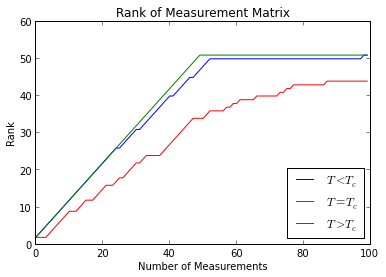
\includegraphics[width=0.5\linewidth]{Ranks.png}
\end{center}
\caption{Measurement matrix ranks at various temperatures}
\end{figure}
This would seem to indicate that the critical state offers some advantage over its
neighboring phases in its ability to transmit information located around the model.
In the disordered phase, the small correlation length makes it very difficult to
obtain interactions with distant spins, and in the ordered phase the large interaction
size causes repetitive couplings to all the spins also transmitting redundant information.

Attempting to reconstruct the original signal from these measurement however, has
been far less successful.  Using the Moore-Penrose pseudoinverse to attempt
reconstruction at every step, we were able to calculate reconstruction error
for each measurement (Figure 3).  
\begin{figure}[h]
\begin{center}
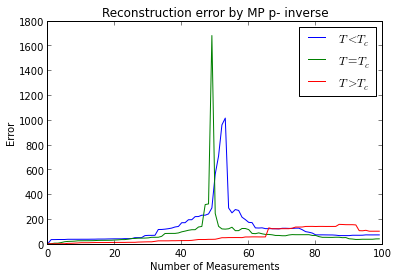
\includegraphics[width=0.5\linewidth]{errors.png}
\end{center}
\caption{Reconstruction error at various temperatures}
\end{figure}
We have far less understanding this figure.  It seems that the critical temperature
is the most numerically unstable of all and especially so just as the matrix reaches
full rank.  As this is the case for the low temperature matrix as well, this may be
a feature of the MP pseudoinverse.  While an $l^1$ minimization would have been more
enkeeping with the original inspiration for this project due to its preferred role
in compressive sensing, it is substantially more difficult to implement and refinements
of the reconstruction will be relegated to subsequent work. As it stands, I believe
the poor quality of the reconstructions is feature of the specific encoding and 
reconstruction scheme used and that further work may yield subsantially more accurate results.

%-------------------------------------------------------------------------------
% PAUL'S SECTION
%-------------------------------------------------------------------------------

\section{Random neural network model}
We considered a neural network model, originally presented by \cite{Sompolinsky1988}, which is a dynamical system describing a network of $N$ randomly connected resitive and capacitive elements.  The equations of motion describing the system are
\begin{align}
	\d{V_i}{t} &= -V_i + \sum_{j=1}^{N} J_{ij} \phi(V_j) \label{eq:m1_eom} + I_i(t)
\end{align}
where $\phi(V_i)$ is an $I/V$ relationship which may be thought of as an ``activity'' proportional to the synaptic current between neurons $i$ and $j$.    One possible choice is a sigmoid function of $V$, i.e. $\phi_i = \tanh\left(\alpha V_i\right)$.  This choice is both biologically motivated as acting to saturate synaptic activity as a function of membrane voltage, as well as mathematically to avoid highly unstable, runaway solutions to eq. (\ref{eq:m1_eom}).  $\alpha$ acts as a control parameter on the turnaround rate of the synaptic activity around $V = 0$; in some sense it controls the ``degree of nonlinearity'' in the system.

The $I_i$ are external inputs into the system.  These may be thought of as sensory inputs in a network model that more approximately represents the structure of a sensory neural network.  They may be included here, anyway, to experiment with estimation of the external inputs using synchronization.

The matrix $J_{ij}$ describes the connectivity in the network; in this particular model, $J_{ij}$ is chosen to be a Gaussian random matrix with elements distributed according to the statistics
\begin{align}
	\exval{J_{ij}} = 0, \quad \exval{J_{ij}J_{kl}} = \frac{\tilde{J}^2}{N} \: \delta_{ik}\delta_{jl} \label{eq:m1_stats}
\end{align}
with zero on the diagonals to eliminate self-coupling terms.  This means synaptic connections are totally decorrelated and, in general, asymmetric.  This also means that, on average, half of the connections are inherently inhibitory and half are excitatory.  If $J_{ij}$ were symmetric, (\ref{eq:m1_eom}) would describe a system that relaxes to a global minimum of an energy function; with asymmetric couplings the dynamics are that of a spin glass, which in general have nonrelaxational and possibly chaotic behavior.

A detailed mathematical treatment of this model in the limit of large $N$ is given in \cite{Sompolinsky1988}.  The result is that under the replacement $\alpha \rightarrow \tilde{J}$ in the expression for $\phi$, the model undergoes a ``phase transition'' when the control parameter $\tilde{J}$ reaches a critical value of 1.  This is manifest in the structure of the attracting solution manifold in the $\{V_i\}$ state space, which acquires at least one positive Lyapunov exponent; in other words a family of chaotic solutions to (\ref{eq:m1_eom}) appears.

\section{Dynamical synchronization technique}
Dynamical synchronization is a widely-used technique for performing state estimation in systems which can be adequately described by dynamical systems \cite{Abarbanel2009}.  In this technique, the model equations are coupled to a set of data through a linear term as
\begin{align}
	\d{x_i}{t} = f_i(x) + \sum_{j} g_{ij} \left(y_j - x_j\right)
\end{align}
where $x(t)$ and $y(t)$ are the model and the data trajectories, respectively, and $g_{ij}$ is a set of positive coupling constants.  In practice, only a subset of the couplings will be nonzero (corresponding to the components of the system which can be measured) and the matrix $g_{ij}$ is diagonal, since in this scheme there is no obvious advantage to coupling different components of the system to each other\footnote{In a further examination of the model, we hope to test a coupling scheme which couples components to each other in time-delayed coordinates.  Because the components are coupled through the dynamics, the time-delayed trajectories can provide information about each other and enhance the scheme by coupling unmeasurable components to the data.}.  The linear term acts like a driving force on $x$, dragging the coupled components of the dynamics towards the observed values $y$.

It may be possible for \emph{all} the components of a model to synchronize to a data set if enough measurements are made, and if the coupling strenghts are large enough.  What constitutes ``enough'' comes on a case-by-case basis.  Roughly, what is required is for the linear terms to regularize the solution manifold by driving the value of the largest Lyapunov exponent in the coupled system to a non-positive value.

The typical procedure in this kind of analysis is to produce a set of (possibly noisy) dummy data using the model, and couple this back into the model itself.  The coupled ``observer'' model is then integrated forward in time, as usual. This allows one to evaluate whether or not the model can synchronize to a data set which is representative of the dynamics in a controlled setting.  One requires a metric of success to make the call, which might be something as simple as
\begin{align}
	M = \frac{1}{T} \int_0^T dt \; \left(x_i^\text{(obs)}(t) - x_i^\text{(data)}(t)\right)^2
\end{align}
in which case a smaller $M$ means a more successful attempt at synchronization.  This kind of procedure is sometimes referred to as a twin experiment.

\subsection{Numerical analysis}
We examined the model for $N=256$ neurons with a single instantiation of $J_{ij}$, with all $I_i=0$, for now at least.  Ideally, we would like to scale up the simulation size to a larger $N \sim 1000$, and to gather statistics about an \emph{ensemble} of models parameterized by different instantiations of $J_{ij}$.  However, limited by time, we now present said results as at least a preliminary examination of the model.

First, we performed a comparison of numerical results to the analytic results of \cite{Sompolinsky1988}.  For a single randomly drawn instantiation of $J_{ij}$, (\ref{eq:m1_eom}) was integrated forward in time using the \texttt{LSODA} solver in \texttt{scipy.integrate}.  The initial conditions were drawn randomly from a ball of radius 1 centered about the origin $V_i=0$.  To examine the behavior of $\Delta(t)$ alongside the phase space trajectories, it was assumed that the steady state of the system was ergodic so as to allow the replacement
\begin{align*}
	\exval{V_i(t_0)V_i(t+t_0)} \rightarrow \int_{t_0}^{T-t} dt^{\prime} \; V_i(t^{\prime}) V_i(t+t^{\prime})
\end{align*}
(up to an overall scale factor) where $T-t_0$ is the length of the recorded time series.  In other words, the ensemble average was replaced with a time average.  This was necessary because only a single instantiation of $J_{ij}$ was used, and the LHS is an ensemble average over the distribution of $J_{ij}$.  In the analysis, the average value
\begin{align}
	\bar{\Delta}(t) \equiv \frac{1}{N} \sum_i^N \Delta_i(t)
\end{align}
was computed to assess the overall behavior of the system, which for large $N$ should be representative of the behavior of most of the components of the network.

The critical value of $\tilde{J}$ was reckoned to be the value where $\bar{\Delta}$ ``smoothed out'' over $t$.  Below this value, the correlation oscillates with the frequency of the system when it is executing a limit cycle trajectory; well above this value the surface becomes very rough, and peaks sharply at $t=0$.  This is where the solution is chaotic, so time correlations along the trajectory decay quickly.

Finding the critical value of $\tilde{J}$ provided us with a place to examine the effect of criticality on synchronization. The observer system looks like
\begin{align}
	\d{V_i}{t} = -V_i + \sum_{j=1}^{N} J_{ij} \tanh(\tilde{J} V_j) + g_i (V^{(D)}_i - V_i)
\end{align}
where $M$ elements of $g_i$ are nonzero, corresponding to the $M$ measured components of the system (corresponding to the $M$ data time series $V_i^{(D)}$).  This was, again, integrated forward step-by-step over the data points, and compared to the data trajectory.

\subsection{Results}
$\bar{\Delta}(t)$ was calculated for various values of $\tilde{J}$, near to and far from the point where the system becomes chaotic.  The transition appeared to occur at about $\tilde{J} = 1.252$.  Notice this is \emph{not} $\tilde{J}=1$; however, it can be argued that for finite $N$, the solution does not immediately become chaotic but undergoes a period doubling cascade whose width (over $\tilde{J}$) shrinks as $N$ grows (see \cite{Sompolinsky1988}).  In this regard, our numerical result thus shows some agreement with the analytical calculation.

\begin{figure}[p]
	\centering
	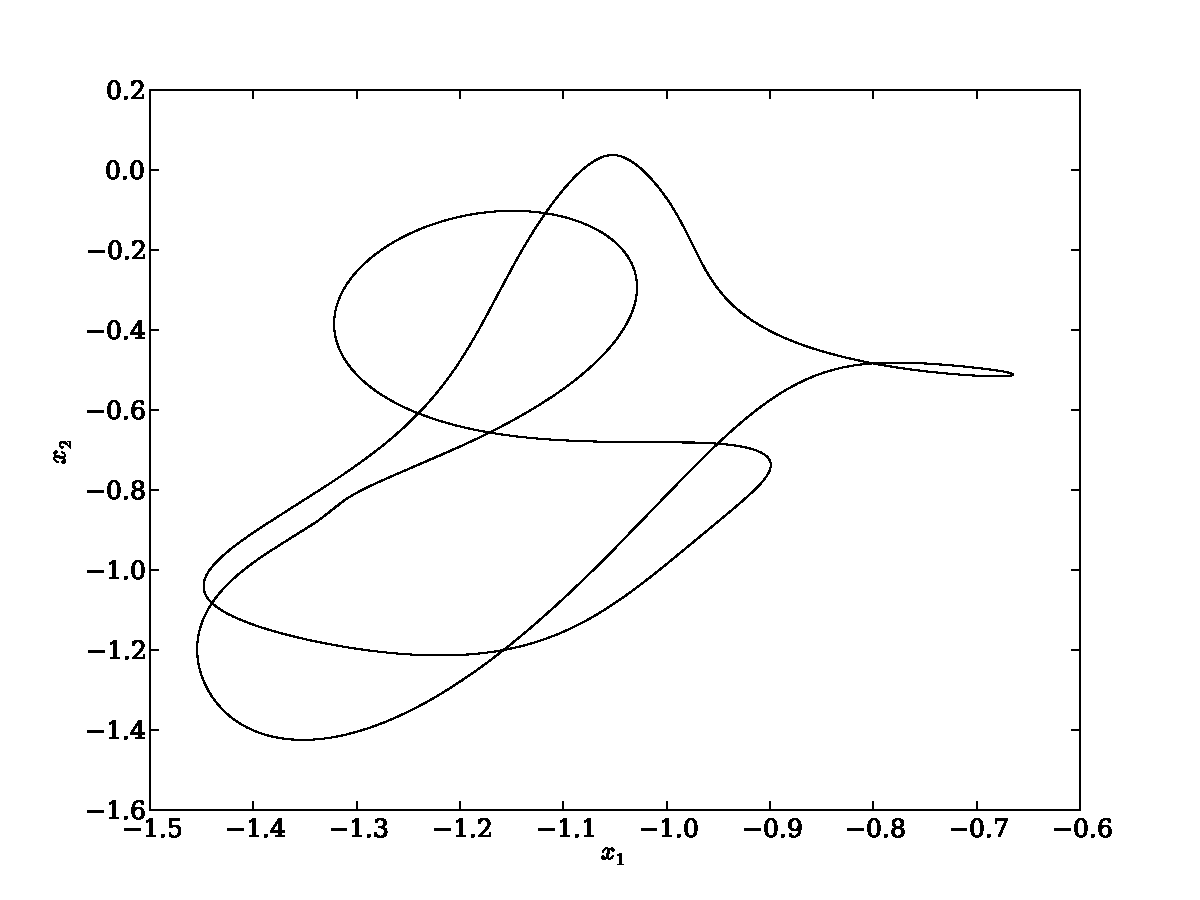
\includegraphics[width=0.9\textwidth]{paul_figs/J_1_23}
	\caption{$J=1.23$, phase space trajectory}
	\label{fig:first_pstcorr}
\end{figure}
\begin{figure}[p]
	\centering
	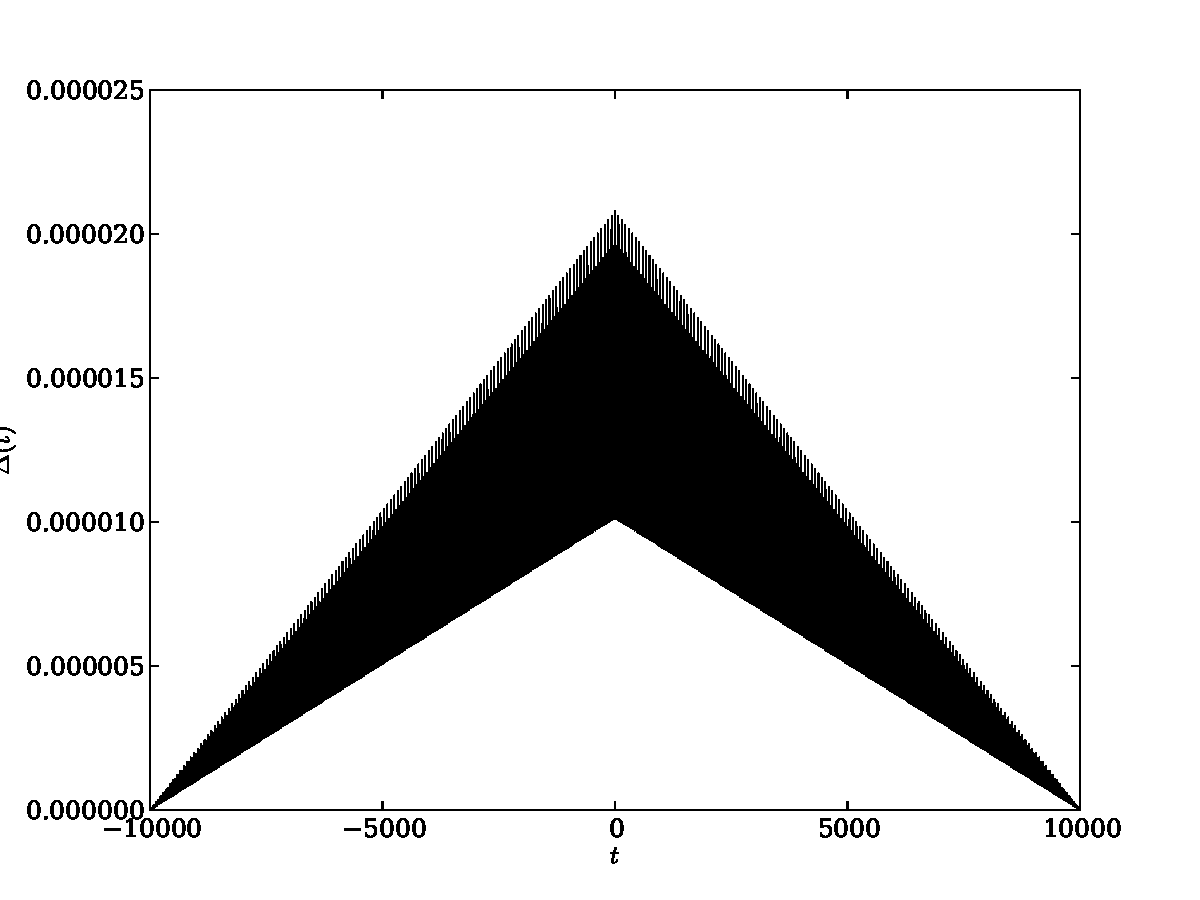
\includegraphics[width=0.9\textwidth]{paul_figs/tcorr_J_1_23}
	\caption{$J=1.23$, time correlation}
\end{figure}
\begin{figure}[p]
	\centering
	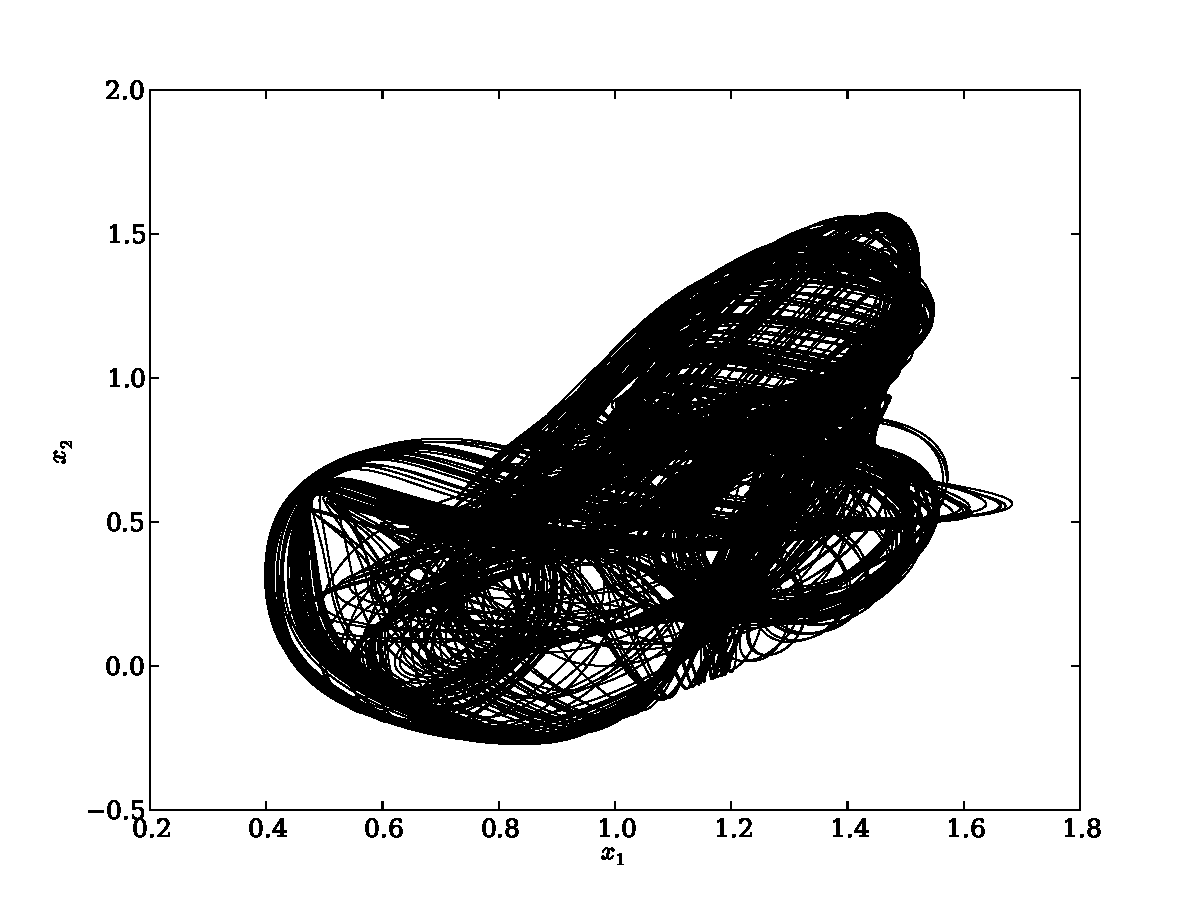
\includegraphics[width=0.9\textwidth]{paul_figs/J_1_252}
	\caption{$J=1.252$, phase space trajectory}
\end{figure}
\begin{figure}[p]
	\centering
	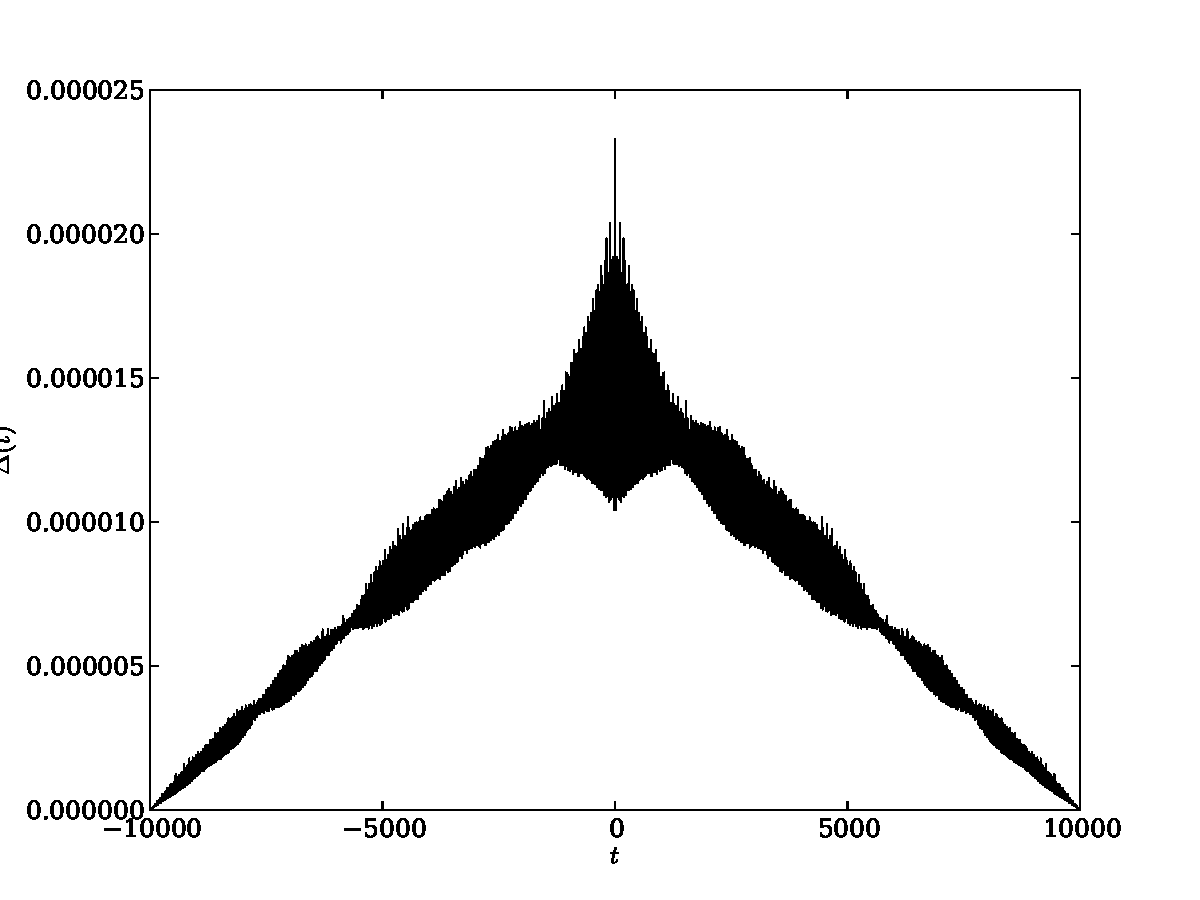
\includegraphics[width=0.9\textwidth]{paul_figs/tcorr_J_1_252}
	\caption{$J=1.252$, time correlation}
\end{figure}
\begin{figure}[p]
	\centering
	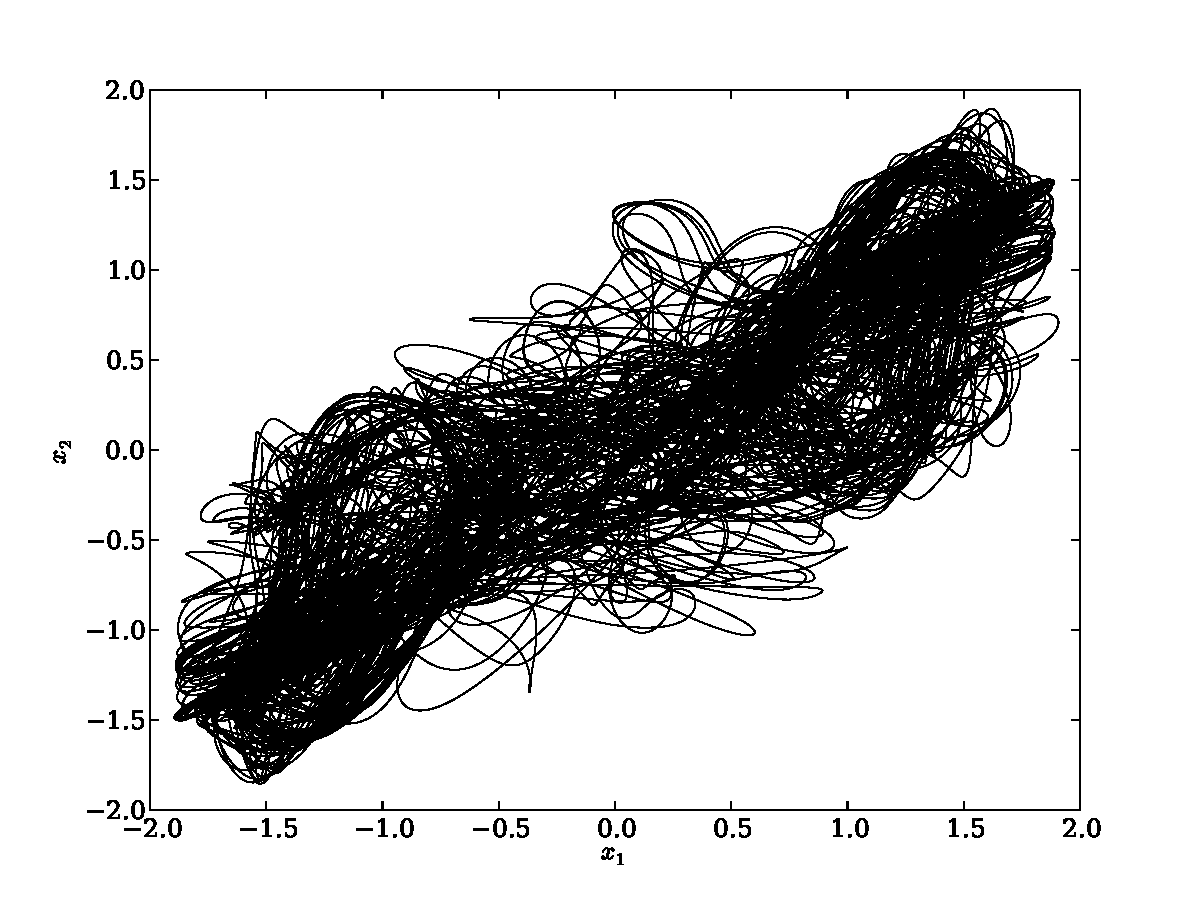
\includegraphics[width=0.9\textwidth]{paul_figs/J_1_3}
	\caption{$J=1.3$, phase space trajectory}
\end{figure}
\begin{figure}[p]
	\centering
	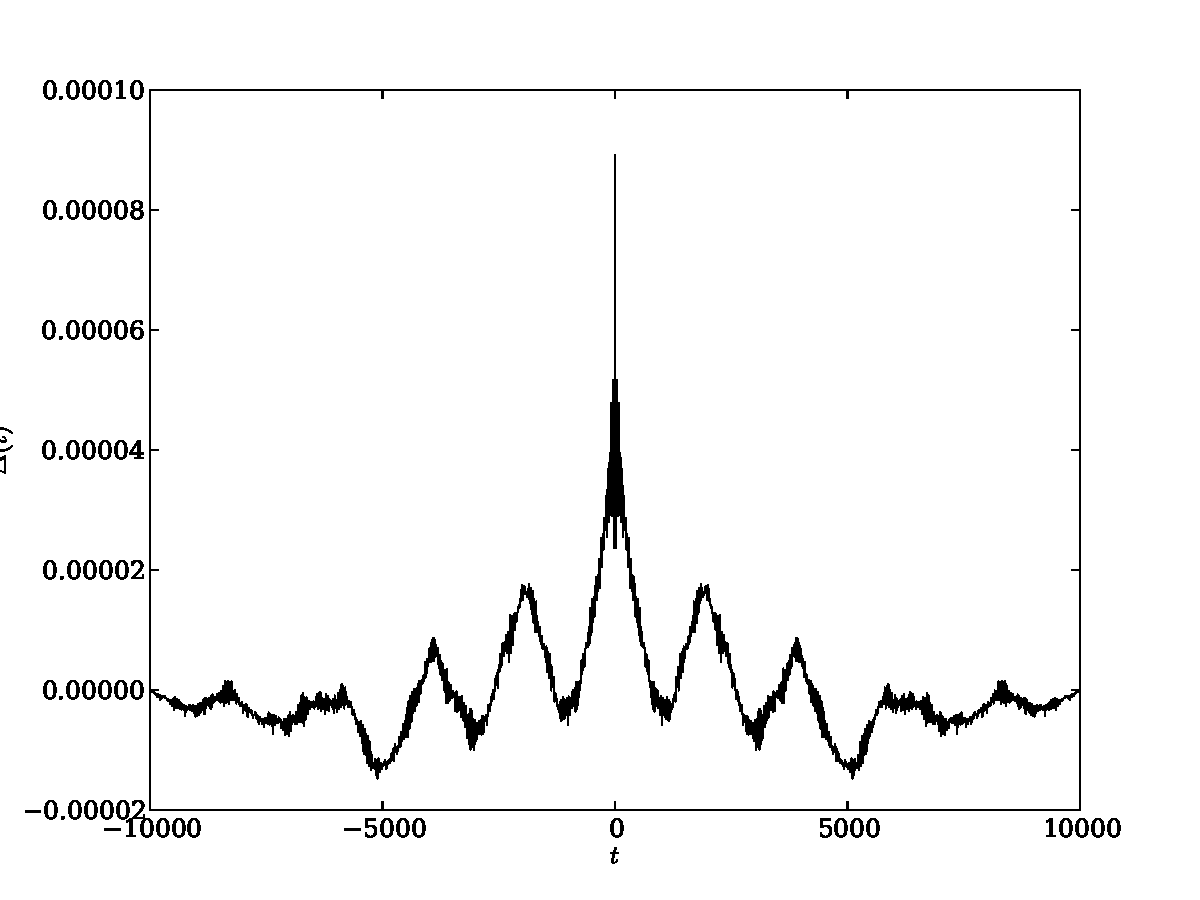
\includegraphics[width=0.9\textwidth]{paul_figs/tcorr_J_1_3}
	\caption{$J=1.3$, time correlation}
\end{figure}
\begin{figure}[p]
	\centering
	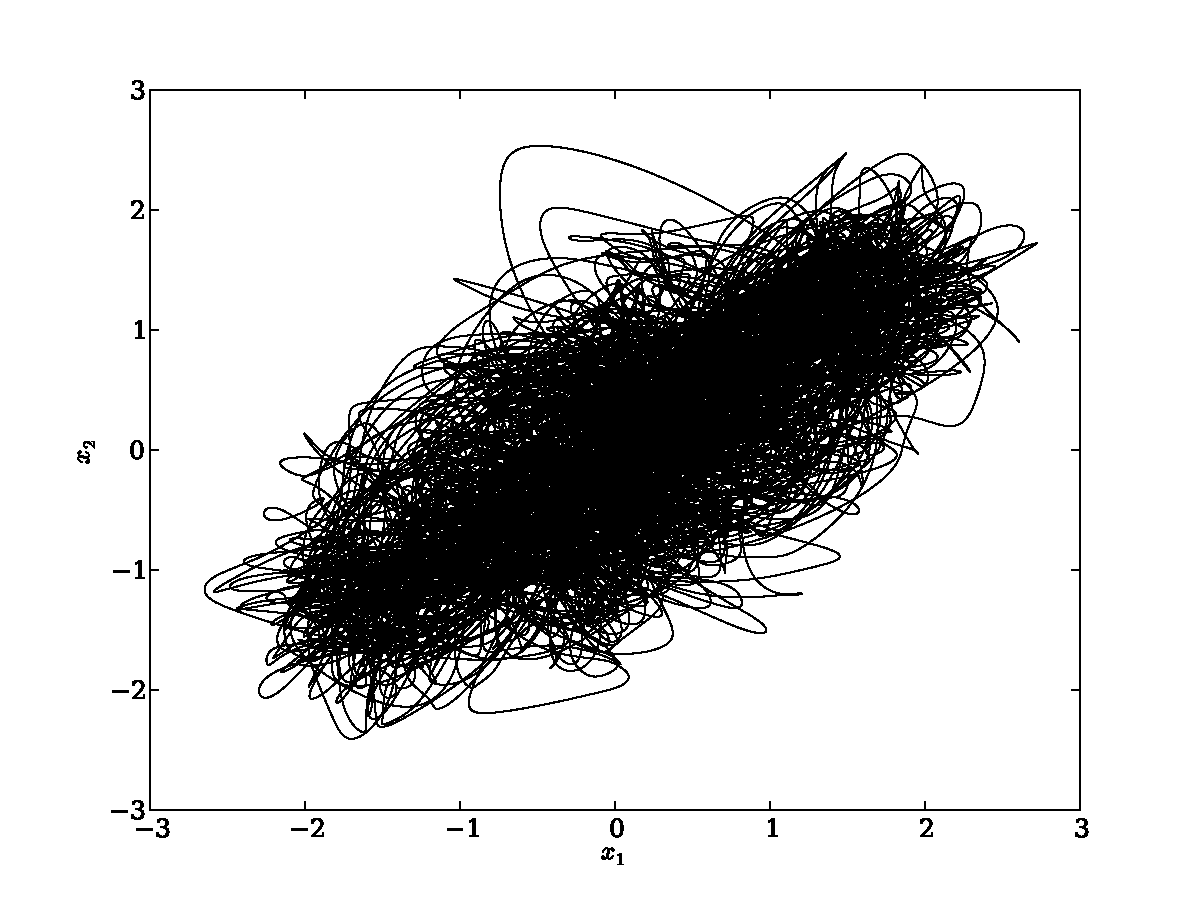
\includegraphics[width=0.9\textwidth]{paul_figs/J_1_4}
	\caption{$J=1.4$, phase space trajectory}
\end{figure}
\begin{figure}[p]
	\centering
	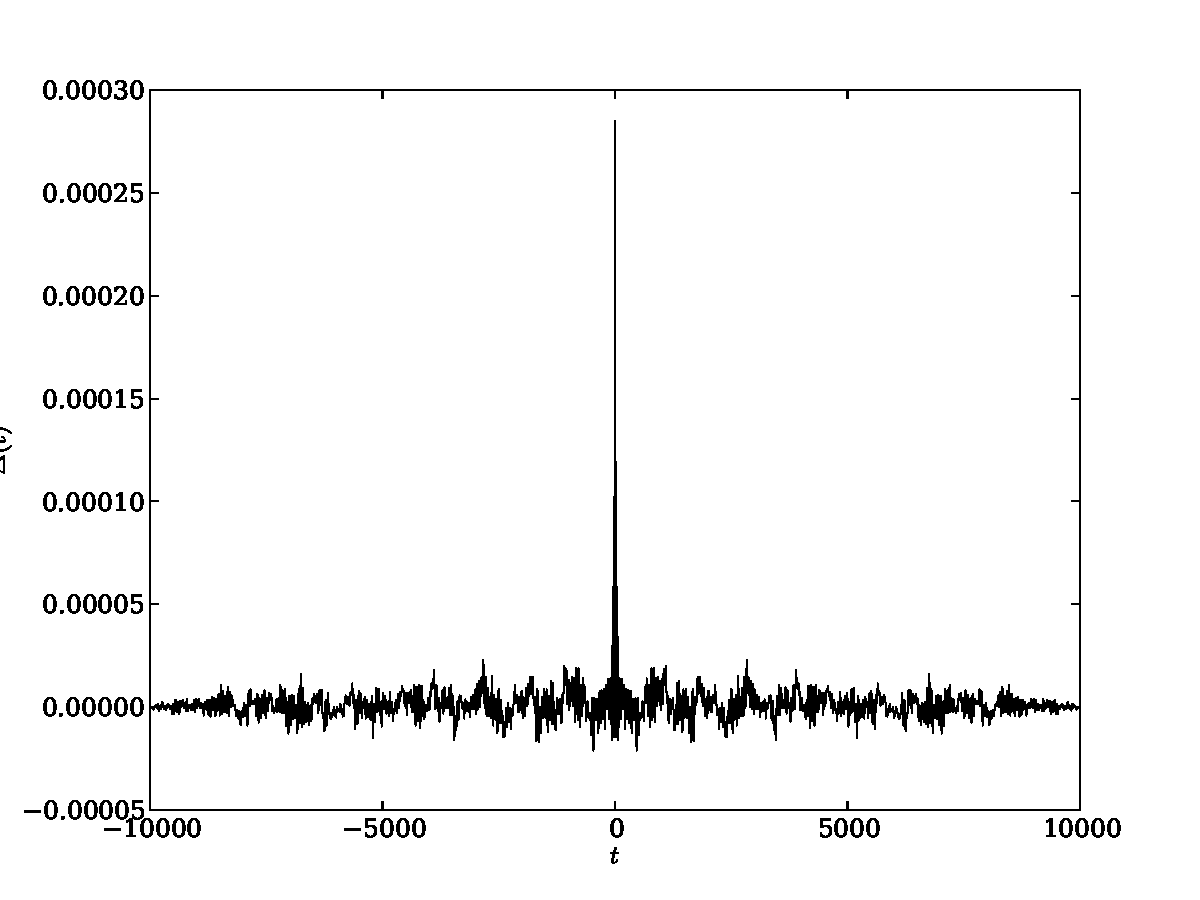
\includegraphics[width=0.9\textwidth]{paul_figs/tcorr_J_1_4}
	\caption{$J=1.4$, time correlation}
	\label{fig:last_pstcorr}
\end{figure}

See figs. \ref{fig:first_pstcorr}-\ref{fig:last_pstcorr} for various comparisons of the phase space trajectory (projection onto two components) to $\bar{\Delta}(t)$.  At $J=1.2$, there is a limit cycle solution; once $J=1.23$, a period-doubling has occurred which is also apparent in $\bar{\Delta}$.

The behavior at $J=1.252$ has already become quite complex.  Notice the structure of the attractor in phase space, as well as that of $\bar{\Delta}$ which has flattened quite a bit by this point. Many individual components of the system, in fact, have become completely flat (not shown).  Beyond this, at $J=1.3$, $\bar{\Delta}$ is showing ``in-between'' behavior where it is oscillating, but also quickly decaying as the model is approaching chaotic behavior.  At $J=1.4$, the model seems to have clearly become chaotic.

\begin{figure}[p]
	\centering
	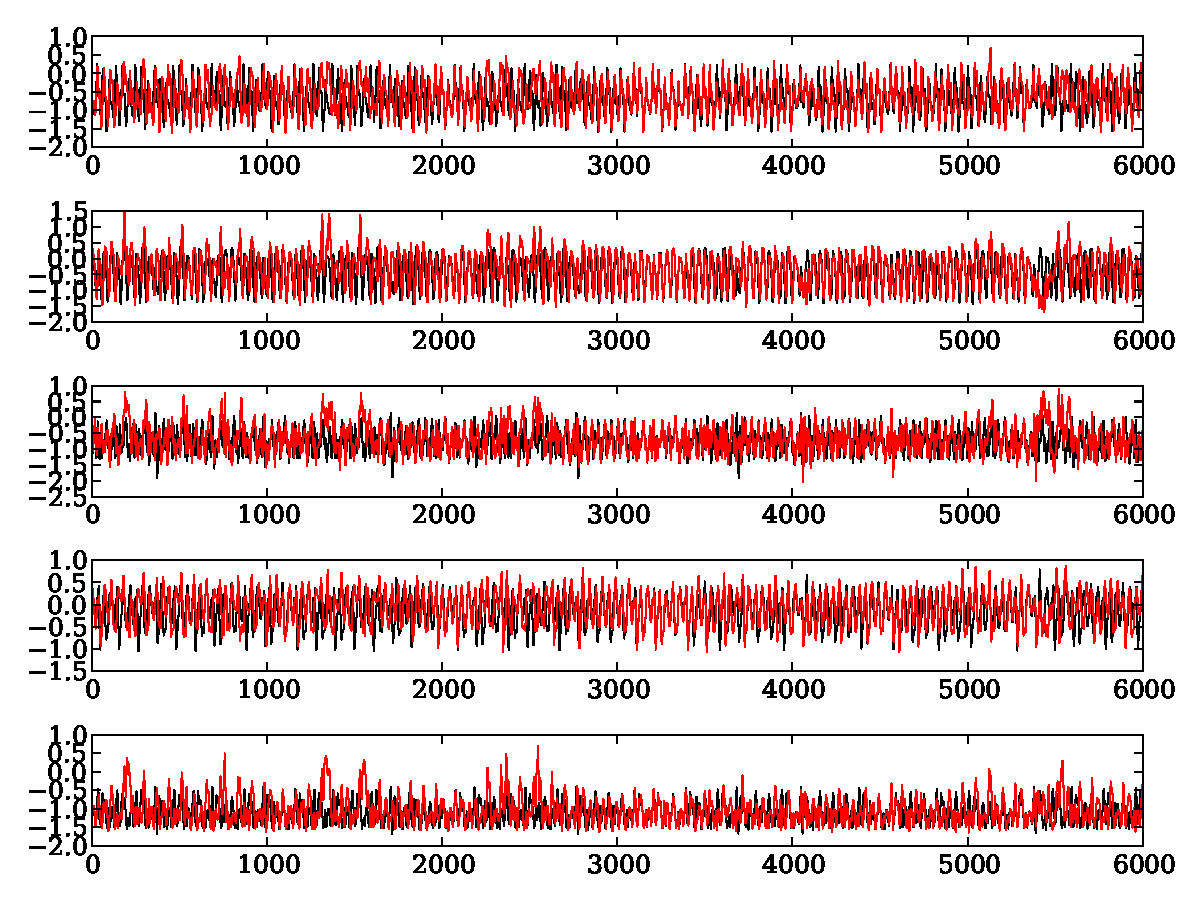
\includegraphics[width=0.9\textwidth]{paul_figs/sync_J_1_252_g_0_3}
	\caption{Synchronization twin experiment, with data in black and observer in red.}
	\label{fig:twinex}
\end{figure}

It seems like $J=1.252$ is a good place around which to test our hypothesis.  Unfortunately, due to time constraints, we got as far as coding the coupled model and calculating some sample trajectories, but no conclusive results have been obtained yet. See fig. \ref{fig:twinex} for a sample of the outcome at $\tilde{J}=1.252$ and with $N=200$ components of the system coupled to the data.

\subsection{Discussion}
The behavior of $\bar{\Delta}$ is encouraging for the future progress of this project.  It is important that the correlations in many components of the system seem to flatten completely near the critical value of $\tilde{J}$.  This kind of behavior is exactly what is expected out of criticality, where correlation lengths in the system (in both the time and space domains) are expected to diverge.  Ideally, this will produce the effect of maximizing the ability of the system to synchronize near the critical point.

The resulting $\bar{\Delta}$ at other values of $\tilde{J}$ confirm expecations, as well.  On limit cycles, time correlations \emph{should} be periodic since the system is periodic over the period of the cycle.  Additionally, we expect chaotic behavior to quickly degrade correlations and produce very rough, jagged behavior otherwise (which is essentially due to the fractal dimension of the attractor).

Our future direction with this model is to examine its synchronization capabilities both near and far from the critical point, using the aforementioned procedure or, in the future, using time-delayed coordinate information to couple unmeasured components of the model to the data.

%-------------------------------------------------------------------------------
% REFERENCES
%-------------------------------------------------------------------------------
\bibliographystyle{unsrt}
\bibliography{refs}



\end{document}
